\documentclass[../main.tex]{subfiles}
\begin{document}

%% The second part compares Toivonen's bounds and d-bound sample size by performing experiments
%% on frequent itemsets.

\section*{Part II -- Experimental Evaluation}
\setcounter{section}{2}
\setcounter{subsection}{0}
\addcontentsline{toc}{section}{Part II -- Experimental Evaluation}

\subsection{Introduction}
\label{sec:II_intro}

In the second part of the essay we will discuss the results of an experimental study performed on mining of frequent itemsets.
The goal of the experiments is to compare Toivonen's bounds to the d-bound.
How big of a sample do each of the bounds prescribe, and how good are the approximate results.
The sample sizes can be easily calculated by equations \ref{eq:toivonen} and \ref{eq:d-bound}.
We measure the approximate results by comparing the likeliness of the frequent itemsets found from the sample.


During the experiments we vary the parameter pair $(\epsilon, \delta)$ accordingly for both bounds.
In addition to the parameter pair, Toivonen's bounds also uses $\mu$.
Furthermore, we use data sets of sufficiently large size to be certain that the samples will always be smaller than the data set.


The minimum sample size according to Toivonen's bounds can be seen in equation~\ref{eq:toivonen}.
Furthermore, for the calculated sample size $\abs{S}$, Toivonen's bound lowers the threshold by equation~\ref{eq:toivonen_threshold}.

\begin{tabularx}{\textwidth}{X X}
    {\begin{align} \label{eq:toivonen}
        &\abs{S} \ge \frac{1}{2\epsilon^{2}} \ln \frac{2}{\delta}
    \end{align}}
     & 
    {\begin{align} \label{eq:toivonen_threshold}
        &\sqrt{\frac{1}{2\abs{S}}\ln\frac{1}{\mu}}
    \end{align}}
\end{tabularx}

The mimum sample size according to the d-bound can be seen in equation~\ref{eq:d-bound}.
Besides the parameters, there is a constant $c$ in the equation.
We follow the suggestion from \citeauthor{Riondato2012} experiments \cite{Riondato2012}, and fix $c$ at \num{0.5}.
\begin{align} \label{eq:d-bound}
    \abs{S} \ge \min \left\{ \abs{D}, \frac{4c}{\epsilon^{2}}\left( d + \log \frac{1}{\delta} \right) \right\}
\end{align}


\subsection{Experimental Setup}
\label{sec:II_setup}

The experimental setup is based on the experiments described in the works by \citeauthor{Riondato2015} \cite{Riondato2015},
the book \citetitle{Leskovec2014mining} \cite{Leskovec2014mining},
and the slides of the lectures given during the Big Data course at Utrecht University \cite{Siebes2017fim}.
The following steps describe the process used during the experiments:
\begin{enumerate}[noitemsep]
    \item Inputs: a data set $\mathcal{D}$, and a parameter set $(\epsilon, \delta, \mu)$.
    \item Compute the d-index of the data set $\mathcal{D}$.
    \item Based on the parameters, compute Toivonen's and the d-bound sample sizes.
    \item \label{enum:sampling} Mine using sampling, once for Tiovonen's bound and once for the d-bound:
        \begin{enumerate}[noitemsep]
            \item Draw (with replacement) a sample of the computed size.
            \item Compute the set $\FI$ of frequent itemsets on this sample.
        \end{enumerate}
    \item \label{enum:compare} Compare the found frequent itemsets $\FI$ on their likeliness.
    \item Repeat step \ref{enum:sampling} and \ref{enum:compare}, 10 times for each set of parameters --- we want to minimize the effect of the random sampling.
\end{enumerate}

The likeliness is calculated by comparing the two frequent itemsets that were found in the bounded samples.
We simply calculate the intersection of the two itemsets.
Therefore we get an itemset of all items that are in both frequent itemsets.
The size of this intersection (absolute and relative) is presented in the results.


We used data sets from the FIMI repository \cite{FIMI2003}.
Similar to the paper by \citeauthor{Riondato2015}, we use the `blow up' trick to replicate the data set a number of times,
so that it is more representable compared to the sizes of modern data sets \cite[Section~5]{Riondato2015}.
The sizes in table~\ref{tbl:experiment_sets} reflect the sizes of the data sets after applying the `blow up' trick.

\begin{table}[h]
    \centering
    \begin{tabular}{l r r r}
        \hline
        Name & Replication factor & Size $\abs{\mathcal{D}}$ & $d$-index \\
        \hline
        connect & \num{250} & \num{16889250} & \num{43} \\
        pumsb\_star & \num{250} & \num{12261500} & \num{59} \\
        \hline
    \end{tabular}
    \caption{Data sets characteristics}
    \label{tbl:experiment_sets}
\end{table}

The three parameters were varied accordingly:
$\epsilon = \left\{ 0.01, 0.015, 0.02, 0.025 \right\}$,\\
$\delta = \left\{ 0.01, 0.05, 0.1 \right\}$, and
$\mu = \left\{ 0.01, 0.05, 0.1 \right\}$.
Varying the three parameters, and repeating each sampling round 10 times for the parameter set,
results in a grand total of \num{720} experiment runs.


The experiments and mining of frequent itemsets were implemented in Python,
using \citeauthor{Borgelt2016}'s PyFIM library \cite{Borgelt2016}.
The implementation of the experiments can be found on GitHub \cite{Robeer2017}.


\subsection{Results}
\label{sec:II_results}

\begin{figure}[bh]
    \centering
    \begin{minipage}[b]{0.48\textwidth}
        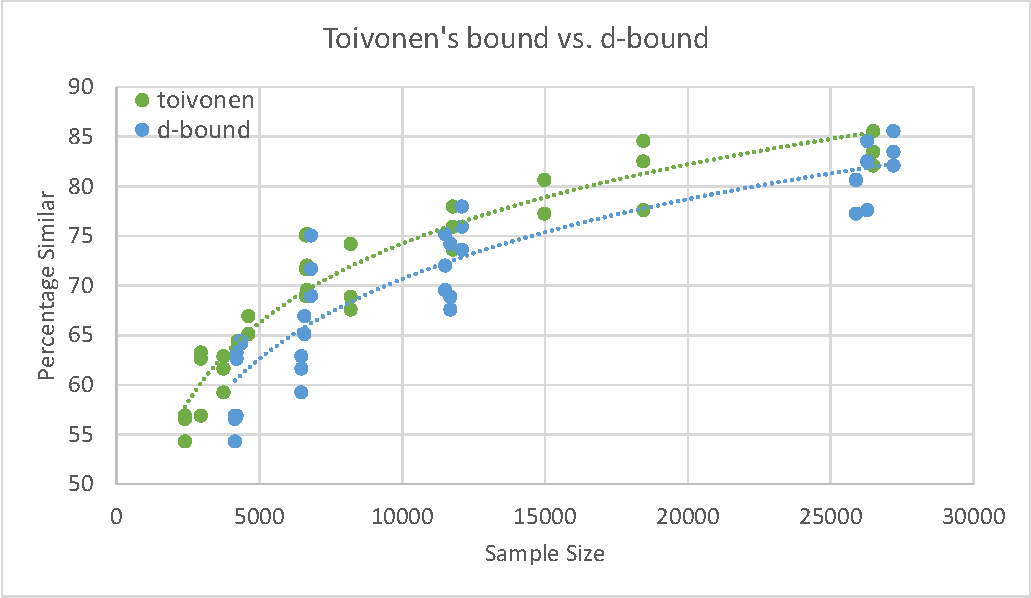
\includegraphics[width=\textwidth]{chart_connect_dat.pdf}
        \caption{Data set \emph{connect}}
        \label{fig:connect}
    \end{minipage}
    \hfill
    \begin{minipage}[b]{0.48\textwidth}
        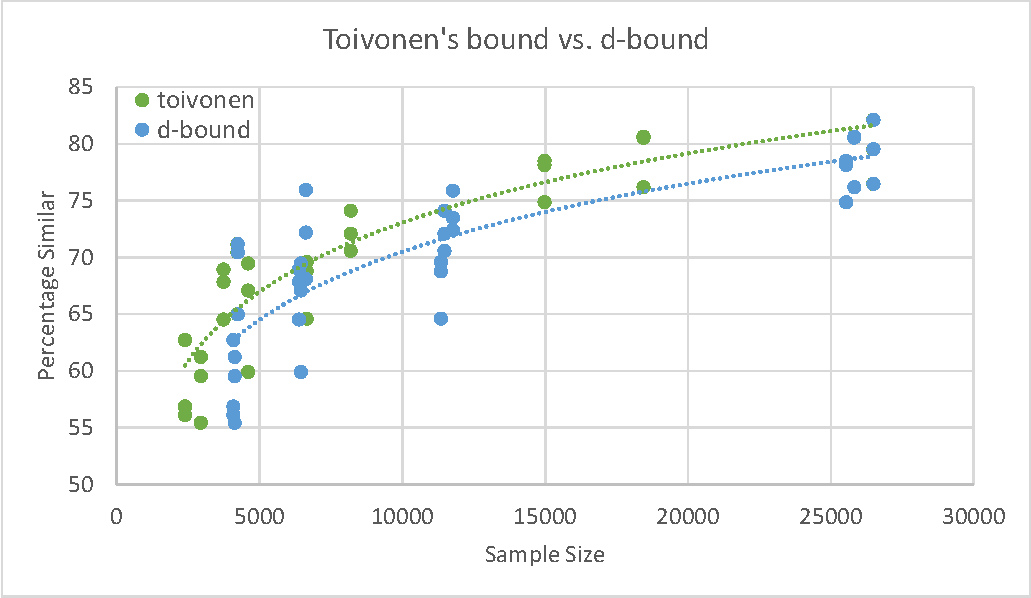
\includegraphics[width=\textwidth]{chart_pumsb_star_dat.pdf}
        \caption{Data set \emph{pumsb\_star}}
        \label{fig:pumsb_star}
    \end{minipage}
\end{figure}

In the experiments we measured the samples sizes by Toivonen's and the d-bound,
the size of the frequent itemsets that were found,
and how many itemsets the frequent itemsets share (their likeliness).
The results of the experiments are summarized in figures \ref{fig:connect} and \ref{fig:pumsb_star},
and in table~\ref{tbl:results}.


We observed that the smaller the parameters $(\epsilon, \delta, \mu)$ get,
the larger the sample sizes are.


Figure~\ref{fig:connect} and figure~\ref{fig:pumsb_star} show the relation between the chosen sample sizes,
and the percentage in which the two resulting frequent itemsets are similar.
If two frequent itemsets are \SI{100}{\percent} similar, every itemset from one of them can be found in the other.
Please note, that to show both samples sizes in the same graph we scaled down the d-bound sample sizes.
The scaling factor is more or less equal to the largest d-bound sample size over the largest Toivonen's sample size.

\begin{table}[h]
    \centering
    \begin{tabular}{l r r r r r}
        \hline
        Data set & & Toivonen's $\abs{S}$ & d-bound $\abs{S}$ & Toivonen's $\abs{\FI}$ & d-bound $\abs{\FI}$ \\
        \hline
        connect & \emph{min} & \num{2396}  & \num{144968} & \num{1526260} & \num{1574977} \\
                & \emph{max} & \num{26491} & \num{952103} & \num{1715820} & \num{1597605} \\
        \hline
        pumsb\_star & \emph{min} & \num{2396}  & \num{196168}  & \num{645} & \num{651} \\
                    & \emph{max} & \num{26491} & \num{1272103} & \num{735} & \num{656} \\
        \hline
    \end{tabular}
    \caption{Summary of experimental results}
    \label{tbl:results}
\end{table}


\subsection{Conclusion}
\label{sec:II_conclusion}

The samples sizes proposed by the d-bound are significantly larger than the sample sizes proposed by Toivonen's bound.
However, the size of the resulting frequent itemsets $\FI$ is very close.
Although the sample of the d-bound is larger, the found frequent itemset size lies close to that of Toivonen's sample.


Figures \ref{fig:connect} and \ref{fig:pumsb_star} show that an increase in the sample size leads to a higher likeliness between the found frequent itemsets.
They will probably hardly ever be completely similar.
Nonetheless, if we do pick a bigger sample, the likeliness of the two frequent itemsets will only be fractionally better.

Furthermore, what the figures do not show, but what can be seen from table~\ref{tbl:results},
and previous experimental results \cite{Goethals2003fimi, Borgelt2012} is the larger the sample size gets, the more time is needed to mine for frequent itemsets.
When applying such bounds in practice, the trade-off between the available time, resources, and accuracy should be made with care.

\end{document}